\section{Background}
In this section, we first introduce the brief background, including virtualization and RDMA. 

\subsection{Cloud and Virtualization}
Cloud is popular for its efficiency and elasticity, and virtualization is the basic for clouds. Nowadays, VMs and containers are both common virtual instances in clouds. VMs need emulate whole virtual hardware environments for guest operation system with hypervisor (kernel-space). So, applications in VMs is isolated by guest OS with more security but higher overhead. Containers are shared with the host OS but with run-time isolation. So, containers have low overhead and fast boot-up time.

For software virtualization of I/O devices, there are two main choices for where to emulate the device: kernel-space and user-space. In kernel-space, the codes of device emulation are inserted into hypervisor or host kernel. Compared to kernel-space, there are three advantages for user-space: first, the attack surface is limited for user-space with minimal inserted code into kernel/hypervisor; second, management development is flexible in user-space; third, the inserted codes are often dependent on kernel APIs (e.g. OS architecture, device driver). For example, vhost-net~\cite{vhost-net} is the kernel-space network device and vhost-user-net~\cite{vhost-user-net} has user-mode virtual device. 

\begin{figure}[!ht]
\centering
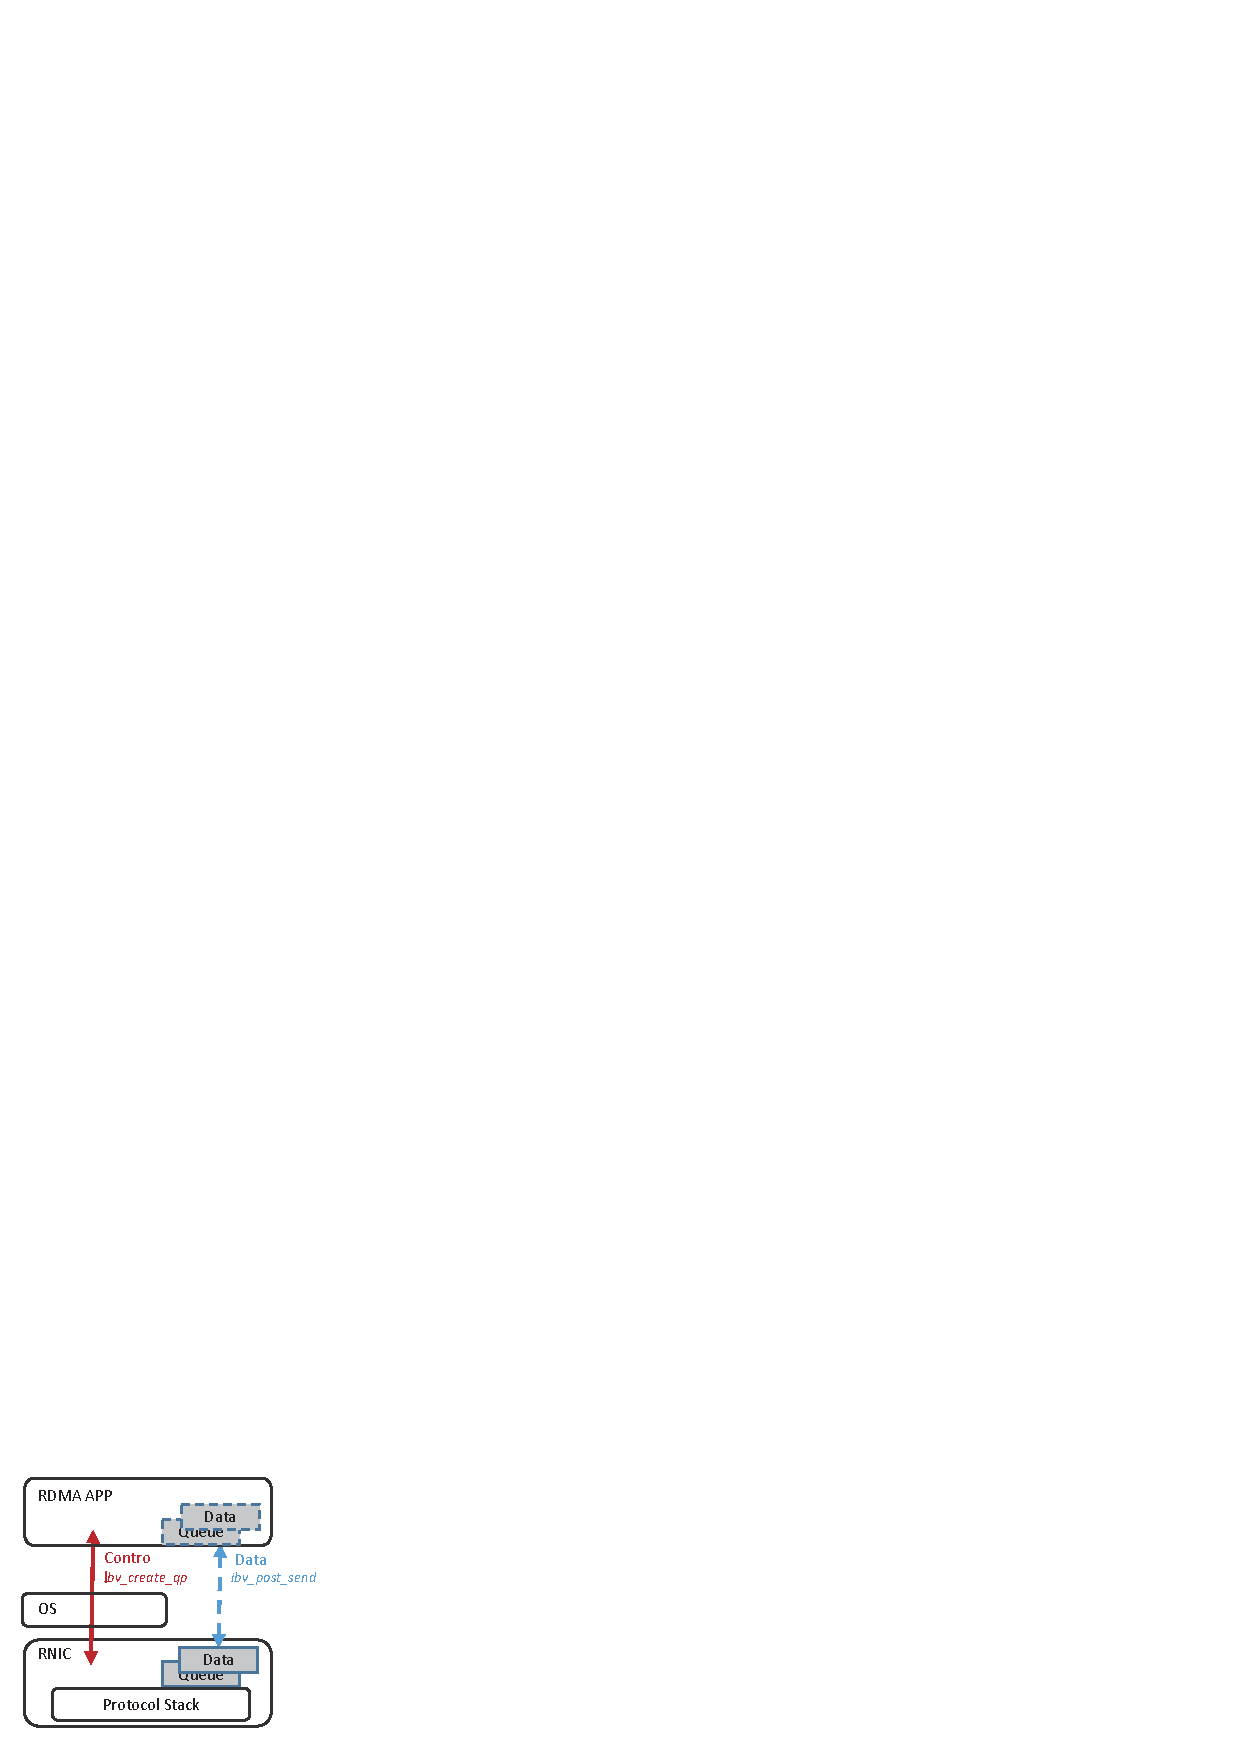
\includegraphics[width=0.8\linewidth]{images/rdma-feat.png}
\caption{Host RDMA Architecture: the control path and data path are separated}
\label{fig:rdma-feat}
\end{figure}

\subsection{RDMA}
As popular high-performance network in supercomputing, RDMA has hardware protocol stack and zero copy technology. With RDMA, applications can bypass the kernel to read and write remote memory data, without the participation of remote CPU. 

% RDMA具备数据零拷贝,绕过内核以及硬件协议栈等特点,因此具备了高性能。在RDMA工作流中,控制路径和数据路径分离。控制路径上,应用创建QP/CQ队列,注册MR等RDMA资源,并将这些资源的ID, Key 或页表缓存到网卡中;在数据路径上,应用可以按门铃寄存器通知网卡,网卡将读取QP中的工作请求,并以零拷贝的方式对本地或远端MR的内容进行读写。数据传输是以零拷贝方式执行的,不需要CPU参与。
RDMA has some features such as zero copy of data, bypassing the kernel and hardware protocol stack, so it has high performance. In the workflow of RDMA, the control path and the data path are separated. In the control path, the application creates QP(Queue Pair), CQ (Completed Queue), registers MR and other RDMA resources, and caches the meta-data to RNIC, such as queue ID, MR key, page tables; In the data path, the application can "press"  the DoorBell register to notify RNIC, then RNIC will read the work request in the QP, read/write the contents of the local/remote MR, and put the completed notifications into the CQ. The data transmission is executed in zero-copy manner and without the CPU.

RDMA can be implemented in different ways, for example, InfiniBand, Roce, and iWARP. However, Verbs is the general interface for applications. Verbs~\cite{verbs} is the basic interface for applications to utilize RDMA. It is similar as socket for traditional network applications. As shown in Figure~\ref{fig:rdma-feat}, RDMA Verbs is also separated to control path and data path as RNIC device. In control path: applications open device and setup the RDMA context. The main resources in RDMA context include Queue Pairs (QPs), Complete Queues(CQs), Memory Regions (MRs). The control verbs include ibv\_create\_qp, reg\_mr;  In data path: applications directly use RDMA resources to transport data and the transport is asynchronous. In specific, applications fillwith the work request into the Send Queue or Receive Queue in a QP, each work request includes the address, size and key of the message. Then the RNIC can execute the operation. The data verbs include ibv\_post\_send and ibv\_post\_recv. Compared control path, data path bypasses the kernel to avoid context switch.

In a RDMA workflow, the communication is based on Queue Pair (QP). The application writes the RDMA work request to the QP, and then ``press''  the RNIC's doorbell register, which is mapped to application when context init, and the RNIC's hardware processor will execute the work request in the QP to forward data. There are two modes for RDMA connect-based communication: one-sided and two-sided. One-sided is that remote server is awareness when client reads or writes its registered memory; Two-sided is that one sends messages after the peer is ready to receive.